%%% Chapter - Extended Summary
%%%%% Wording: ✅
%%%%% Styling: ✅
%%%%% References: ✅
%%%%% Grammar: ✅
%%% --------------------------------------------------------------
\chapter*{Extended Summary}
\label{ch:extended-summary}
The rapid advancement of technology has had a significant impact on various industries, including the entertainment sector, where ticket sales play a crucial role.
The emergence of online ticketing has not only transformed customer behavior by offering a quick, convenient, and user-friendly method of purchasing tickets, but also provided organizers with enhanced efficiency in event planning and management.

A noteworthy development in online ticketing is the ability to reserve specific seats at venues, which offers customers a personalized experience and provides organizers with detailed planning information and effective capacity management.
Additionally, this feature helps reduce the occurrence of ticket fraud, making it highly desirable.

Web-based ticketing with seat reservations has been adopted in numerous sectors, such as entertainment, sports, and travel, as may be seen in the chart~\ref{fig:polaris-market-research}.

However, keeping such solutions relevant to customers in the face of rapid advancements in web technology poses a challenge.
This thesis focuses on utilizing the latest technologies to create a frontend solution for a web-based ticketing and seat reservation application.

\begin{figure}[H]
    \centering
    \caption{Chart showing the share of countries in the market of online ticketing systems.}
    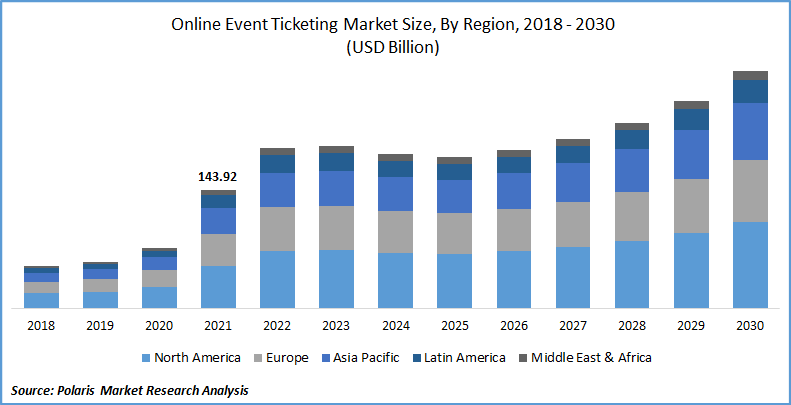
\includegraphics[width=\textwidth]{\FIGDIR/polaris-market-research}
    \source[\citeauthor{online_ticketing_polaris_market_research}]{}
    \label{fig:polaris-market-research}
\end{figure}
\pagebreak

%%% Section - Goals and objectives
%%%%% Wording: ✅
%%%%% Styling: ✅
%%%%% References: ✅
%%%%% Grammar: ✅
%%% --------------------------------------------------------------
\section*{Goals and objectives}
\label{sec:goals-and-objectives}
The main purpose of this work was to create a prototype for a responsive web-based application that enables ticket sales through seat reservations, with a main focus on frontend development.
Built using modern web tools, the app allows potential customers to explore the event map, select their preferred seat, add tickets to cart and complete their order.
While the focus was on the frontend, understanding and analysis of existing ticketing solutions was critical to the development process.
Therefore, the first step was to identify the key components of such a system and then create user stories that guide the design of the user interface.
The goals that define the success of this project are:

\begin{itemize}
    \item Essential elements and functionalities of a web-based ticketing solution with seat reservations were identified.
    \item The application's user interface design was created based on defined user stories.
    \item A responsive web application enabling ticket sales with seat reservations was developed.
    \item The application was deployed in a production environment.
\end{itemize}

%%% Section - Employed methods
%%%%% Wording: ✅
%%%%% Styling: ✅
%%%%% References: ✅
%%%%% Grammar: ✅
%%% --------------------------------------------------------------
\section*{Employed methods}
\label{sec:employed-methods}
This thesis employed a combination of research, comparative analysis, and practical development.
In the initial stages, a comprehensive examination of prevalent ticketing solutions with seat reservation capabilities was conducted.
This examination entailed identifying the essential elements, functionalities, and prevailing patterns of these solutions.

The design phase utilized a comparative analysis of design tools, specifically Adobe XD, Figma, and Sketch.
The decision for their selection was determined by considering their features, user-friendliness, and alignment with project specifications.

In the course of the implementation phase, an extensive examination of documentation was undertaken for the selected web tools and libraries, including React.js, TypeScript, Next.js, Mantine UI, and Tailwind CSS.
These technologies were chosen based on their resilience, appropriateness for the project, and support from the community.

In summary, this thesis relied on a combination of research, comparative analysis, and practical development as its primary methodologies.

%%% Section - Major sources
%%%%% Wording: ✅
%%%%% Styling: ✅
%%%%% References: ✅
%%%%% Grammar: ✅
%%% --------------------------------------------------------------
\section*{Major sources}
\label{sec:major-sources}
This thesis has been informed and enriched by a multitude of resources.
Some have provided deep dives into technical subjects, while others have given guidance on design principles and psychological theory.
Here are the most important sources and how they have contributed to this work:

\subsection*{MDN (Mozilla Developer Network)}
\textit{As a comprehensive resource for web technologies such as HTML, CSS, and JavaScript, MDN has served as the backbone for the technical aspects of this thesis.}\\
\fullcite{mdn_getting_started_with_the_web}\\
\fullcite{mdn_tools_and_testing_client_side_javascript_frameworks_introduction}

\subsection*{Maslow's Motivation and Personality}
\textit{Maslow's theory of human motivation has been instrumental in understanding user behaviors and needs in the context of web development and design.}\\
\fullcite{maslow_motivace_osobnost}

\subsection*{Designing for a Hierarchy of Needs by Steven Bradley}
\textit{This article has seamlessly bridged the gap between Maslow's psychological theory and design practice.}\\
\fullcite{bradley_hierarchy_of_needs}

\subsection*{CSS Tricks}
\textit{This site has been a valuable resource for mastering frontend design and CSS.
It has provided practical tips and solutions for various design challenges, including responsive design, CSS animations and most importantly CSS transforms on SVG elements.}\\
\fullcite{ct_css_tricks_com_transforms_on_svg_elements}

\subsection*{Other important sources}
\fullcite{bs_guide_top_css_frameworks}\\
\fullcite{p_article_react_folder_structure}\\
\fullcite{s_blog_seating_plan_rendering}\\
\fullcite{c_ux_design_the_difference_between_ux_and_ui_design_a_laymans_guide}\\
\fullcite{w_articles_user_stories_a_foundation_for_ui_design}

Each of these resources has played a critical role in shaping the thesis, either by providing technical knowledge, design principles, project management guidelines, or understanding user behaviors and needs.

%%%% Section - Summary
%%%%%% Wording: ✅
%%%%%% Styling: ✅
%%%%%% References: ✅
%%%%%% Grammar: ✅
%%%% --------------------------------------------------------------
\section*{Summary}
\label{sec:summary}
The initial phase of the thesis centered on identifying crucial components of these systems, placing particular emphasis on their user interface.
A critical area of focus involved comprehending user narratives, effectively constructing them, and converting them into tangible features within the user interface.

The interactive map, shopping cart, and order completion functions demonstrate effective responsiveness across various devices, thereby positively impacting the overall user experience.
Although the frontend provides a seamless user experience, there is potential for enhancement and future growth through the implementation of a comprehensive backend system.
The system is designed to be adaptable to different screen sizes, ensuring that users can access the application from various devices without compromising functionality.

Each enhancement would contribute to enhancing the application's robustness, versatility, and user-friendliness, elevating it to the caliber of a professional ticketing system.

At the beginning of the project, four objectives were identified.

The primary objective was to ascertain the significant elements and characteristics of the system employed for ticketing and seating.
These elements were discerned and expounded, particularly the interactive seating chart, the shopping basket, and the order fulfillment procedure.

The second aim of the thesis was to establish a user interface that was grounded in user stories.
These stories were gathered and compiled in a designated chapter, subsequently employed to inform the design of the interface in a separate section.
The ultimate result entailed the creation of the user interface utilizing the Figma tool, which can be found in the appendix.

The third aim of this thesis was to develop a web application that facilitates the sale of tickets with designated seating.
This objective was successfully achieved in the implementation section, wherein a comprehensive account of the application's construction and framework is provided.
The source code for the application has been incorporated in the appendix.

The successful achievement of the fourth objective, which involved deploying the application in the production environment, was realized through a comprehensive process of deploying the application on the Vercel platform.

The objectives have been successfully accomplished, resulting in the development of a fully operational web-based application for ticketing and seating.
This application can be conveniently accessed through the URL \url{https://seating-map.vercel.app/}\.

It demonstrated that the architecture of a project and the appropriate selection of technologies play a crucial role in determining the speed, efficiency, and overall quality of the final product.
The study involved creating a comprehensive ticketing system with a user-friendly interface, which allowed for the practical application of theoretical concepts.
In general, this thesis has conducted an impressive investigation into different aspects of developing web applications, including designing user interfaces and employing frontend development techniques.

The application has laid a solid foundation for future ticketing and seat reservation solutions, with the potential for expansion and improvement to create even more user-friendly and efficient applications.
The research emphasized the importance of designing with the user in mind and the role of new technologies in simplifying complex tasks.

To summarize, this thesis focused on designing a web application that prioritized user experience in frontend development and user interface design.
Additionally, the thesis highlighted the significance of careful planning and organization when managing large-scale development projects.
